\documentclass[a4paper,french,12pt]{article}
\usepackage{babel,amssymb,amsmath}
\usepackage[utf8]{inputenc}
\usepackage{array,colortbl}
\usepackage[T1]{fontenc}
\usepackage{multicol}
%\usepackage{multirow}
%\usepackage[8pt]{pstricks}
\usepackage{textcomp}
\usepackage{fancyhdr}
\usepackage{geometry}
\usepackage{eurosym}
% \usepackage{titling}
%\usepackage{makeidx}
% \usepackage[maxfloats=50]{morefloats}
% \usepackage{hyperref}
\usepackage{ulem}
 
\usepackage{epigraph}
\geometry{rmargin=2.5cm, lmargin=2.5cm, hmargin=2cm, bmargin=2cm}
\pagestyle{plain}
\usepackage[pdftex]{thumbpdf}
%\definecolor{vert}{rgb}{0.25,0.65,0.04}
\usepackage[pdftex,
    bookmarks         = true,
    bookmarksnumbered = true,
    pdfpagemode       = None,
    pdfstartview      = FitH,
    pdfpagelayout     = SinglePage,
    colorlinks        = true,
    linkcolor	      = black,
    pdfborder         = {0 0 0}
    ]{hyperref}
\usepackage{graphicx}
\usepackage[ruled]{algorithm2e}

\newcommand{\HRule}{\rule{\linewidth}{0.5mm}}
% \hypersetup{
% 	pdfauthor = {Philippe \textsc{GAULTIER}},
% 	pdftitle = {Rapport de stage du 17/06/2013 au 23/08/2013},
% 	pdfsubject = {},
% 	pdfkeywords = {},
% 	pdfcreator = {},
% }
% \newcommand{\filename}[1]{\textbf{\#1}}
% \newcommand{\fonction}[1]{\textbf{\itshape{\#1}}} 
% \newcommand{\tabl}[1]{\textbf{\itshape{\#1}}[ ]} 
\begin{document}
\begin{titlepage}
\begin{center}

%Logo

\includegraphics[width=0.4\textwidth]{./logo_ENSIIE.png}~\\[1cm]
\textsc{\huge Ensiie Strasbourg}\\[1.5cm]

%Title
\HRule \\[0.4cm]
{
	\huge \bfseries Rapport de stage
\\[0.4cm] }
\HRule \\[1.5cm]

% Author and supervisor
\begin{minipage}{0.4\textwidth}
\begin{flushleft} \huge
\emph{Auteur:}\\
Philippe \textsc{Gaultier},\\[0.5cm]
\Large élève ingénieur à l'Ensiie Strasbourg
\end{flushleft}
\end{minipage}
\begin{minipage}{0.4\textwidth}
\begin{flushright} \huge
\emph{Maître de stage:} \\
André \textsc{Schaaf},\\[0.5cm]
\Large enseignant-chercheur à l'Université de Strasbourg
\end{flushright}
\end{minipage}

\vfill

% Bottom of the page
{\large Strasbourg, le \today}



%\maketitle
% \theauthor
% \thetitle
% \thedate
% \makeindex
\end{center}
\end{titlepage}

\newpage
{
  \centering
  {
    \vspace{3cm}
    \epigraph{Always code as if the guy who ends up maintaining your code will be a violent psychopath who knows where you live}{Martin Golding}
    \vspace{3cm}
    \epigraph{The road is long and in the end the journey is the destination}{Unknown}
  }
}
\newpage
\textit{\normalsize Dans toute la suite du rapport, l'<<Observatoire>> désigne l'<<Observatoire astronomique de Strasbourg>>
et l'<<Unistra>> ou l'<<UDS>> désignent l'<<Université de Strasbourg>>.}
\setlength{\columnseprule}{0.5pt}
\tableofcontents

\newpage

\section{Introduction}

	L'Observatoire est un établissement de recherche et d'enseignement centré sur l'astronomie, mais c'est aussi un 
	centre de données astronomiques et un centre d'observation réputés mondialement. Il représente la continuité entre
	l'ancien et le nouveau car il dispose d'un riche patrimoine mais est aussi à la pointe de la recherche.  \\
	De plus l'Observatoire est le parfait exemple de l'informatique au service d'autres spécialités scientifiques,
	à la fois dans le domaine de l'expertise, mais aussi sous un aspect éducatif.\\
	Pour toutes ces raisons, j'ai choisi d'effectuer mon stage de deuxième année au sein de l'Observatoire,
	au contact de technologies émergentes à savoir l'Oculus Rift et le rendu graphique 3D moderne.

\section{Présentation de l'observatoire}

	\subsection{Histoire}
		L'Observatoire a été fondé en 1881 sur l'initiative de l'empereur Guillaume II, l'Alsace étant allemande
		à cette époque.\\
		Il est constitué de trois bâtiments : une Grande Coupole, un bâtiment des salles méridiennes avec deux coupoles,
		et un bâtiment à usage de bureau et de résidence.\\
		La Grande Coupole en fer, de 9,2 mètres de diamètre et pesant 34 tonnes2, contient le Grand Réfracteur,
		une lunette de 48,7 cm d'ouverture et 7 m de focale, construite en 1877, la plus grande d'Europe
		au moment de son installation et aujourd'hui (2008) la troisième de France en taille.\\
		Il dispose également d’un riche patrimoine d’instruments et d’ouvrage anciens.
		
	\subsection{Centre de données astronomiques de Strasbourg (CDS)}
	
		Le CDS est à la fois une équipe de recherche et un Service d’Observation.
		Les services de bases de données (SIMBAD, Vizier) et de visualisation (ALADIN) développés par le CDS
		sont utilisés par l’ensemble de la communauté astronomique mondiale. \\
		Celui-ci est l'un des acteurs majeurs du développement de l'Observatoire Virtuel International en astronomie.
		Fin 2008, le CDS a été labellisé TGIR (Très Grande Infrastructure de Recherche) par le Ministère de l'Enseignement Supérieur et de la Recherche, 
		reconfirmé comme Infrastructure de Recherche en 2012, ce qui le range au même niveau que des infrastructures internationales
		comme l’European Southern Observatory ou RENATER à l’échelon national.

	\subsection{Equipe de recherche Galaxies}
	
		L’équipe <<Galaxies>> étudie la formation et l’évolution des galaxies et de notre Galaxie 
		au travers de leurs populations stellaires et de la dynamique des étoiles et de la matière noire. \\
		Elle est impliquée dans la préparation de la mission satellitaire astrométrique Gaia de l’Agence Spatiale Européenne 
		dont le lancement est prévu en 2012 et dans le grand relevé cinématique RAVE. 
	
	\subsection{Equipe de recherche Hautes Énergies} 
	
		L’équipe <<Hautes Énergies>> s’intéresse aux sources galactiques et extragalactiques émettrices en rayons X,
		objets compacts (étoiles à neutron, naines blanches, etc.) et noyaux actifs de galaxies.\\
		Elle est impliquée dans le SSC-XMM, un consortium international de laboratoires sélectionné par l’ESA
		et labellisé par l’INSU comme Service d’Observation, qui est en charge de fournir des catalogues complets
		de sources X observées par le satellite XMM-Newton à la communauté internationale. 

\section{Mon stage}

	\subsection{Objectif}	
	
		L’objectif de ce stage a été centré autour de l'Oculus Rift et a été double:
		\begin{itemize}
		 \item Intégration de l'Oculus Rift à une simulation 3D du système solaire existante,
		 \item Développement d'un programme de visualisation 3D  d'étoiles avec intégration de l'Oculus Rift
		\end{itemize}
		
		J'ai donc travaillé sur deux projets distincts mais néanmoins complémentaires.
		
	    \subsubsection{Skybot 3D}
		Skybot 3D est un logiciel développé en C par l'institut de mécanique céleste et de calcul des éphémérides (IMCCE),
		conjointement avec l'Observatoire de Paris et le CNRS. Son propos est de faire un rendu graphique réaliste
		en 3D à partir des données célestes de ces instituts. En pratique, c'est une simulation 3D du système solaire
		où les échelles sont respectées. Il est encore en développement à la date d'écriture de ce document et
		sa sortie est prévue pour fin 2014.
		Il fonctionne sur toutes les distributions Linux et utilise OpenGL pour le rendu graphique.
		
		Mon travail a donc consisté en l'intégration du rendu Oculus dans cette application, tout en gardant
		le rendu existant.
		
	    \subsubsection{Simulation}
		Ce projet a consisté en la représentation 3D de données provenant du Centre de Données
		de l'Observatoire, décrivant la taille, la position, l'âge et la densité de corps célestes.
		Ces données sont stockées dans des fichiers texte ou binaires, pouvant contenir plusieurs millions
		d'objets.
		
		J'ai eu la liberté de choisir les outils, le langage et les bibliothèques  externes utilisées dans ce programme,
		n'ayant pas de base de code préexistante.
		
		
		
	      
	    
		
	\subsection{L'Oculus Rift}
		
		\subsubsection{Aperçu}
		  L'Oculus Rift est un masque de réalité virtuelle, développé par \emph{Oculus VR}, une entreprise 
		  basée en Californie et rachetée par \emph{Facebook} en mars 2014 pour  2 milliards \$.
		  L'Oculus Rift a été initialement financé via une plateforme de financement collaboratif, \emph{Kickstarter},
		  et a levé 91 millions \$ à cette occasion. \\
		  Il permet une immersion  réaliste dans une scène en trois dimensions, en donnant l'impression d'y être physiquement
		  présent, et crée ainsi une nouvelle expérience
		  utilisateur. \\
		  De plus, son prix est relativement peu élevé (350 \$, environ 300 \euro), ce qui le rend accessible au grand public. \\
		  Pour toutes ces raisons, l'Oculus Rift est adapté à un usage éducatif et professionel, dans des domaines aussi variés
		  que la simulation scientifique, le divertissement, l'éducation, \ldots.
		  
		  La version grand public est prévue pour fin 2014 ou début 2015. J'ai pour ma part travaillé avec la première
		  version du masque, le \emph{DK1}, tandis que la deuxième version, le \emph{DK2} a été distribuée à partir d'août 2014.
		  
		  \begin{figure}[h!]
		    \centering
		      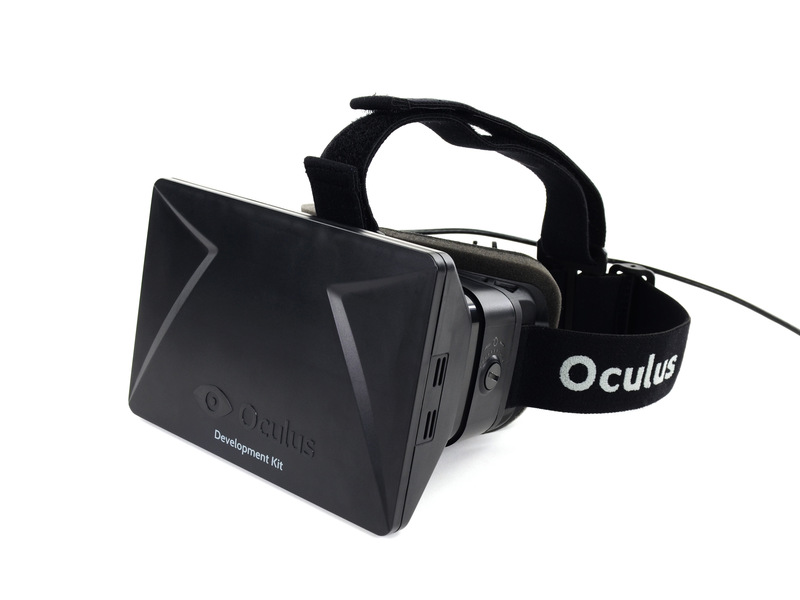
\includegraphics[width=0.3\textwidth]{dk1.jpg}
		    \caption{L'Oculus Rift (DK1)}
		  \end{figure}
		  
		  \subsubsection{Fonctionnement}
		  
			\paragraph{Matériel} ~\\
		    
				L'Oculus Rift est composé de:\\
			      
				\begin{itemize}
				\item Un écran 60 Hz d'une résolution de $1280*800$
				\item Deux lentilles (une pour chaque oeil),
				\item Un gyroscope à 3 axes pour mesurer l'accélération angulaire,
				\item Un magnétomètre à 3 axes pour mesurer les champs magnétiques,
				\item Un accéloromètre à 3 axes pour mesurer l'accélération, y compris gravitationnelle
				\item Un port USB
				\item Un port HDMI
				\end{itemize} ~
			       
				Il est à noter que la résolution de l'écran est à diviser par deux, chaque oeil voyant seulement
				une moitié de l'écran, la résolution effective est donc de $640*800$.
		    
			\paragraph{Logiciel} ~\\
			  
			    L'utilisation de l'Oculus Rift s'effectue au moyen de son SDK, qui permet:\\
			    
			    \begin{itemize}
			     \item D'accéder aux différents capteurs,
			     \item D'accéder aux propriétés du masque (distance inter-pupillaire, hauteur des yeux, \ldots),
			     \item D'appliquer les <<filtres>> au rendu graphique afin d'avoir un rendu réaliste
			    \end{itemize} ~
			    
			    Le SDK est écrit en C++ et possède une API en C.
			    Pour mon stage, j'ai utilisé la version 2.5 puis la version 0.3.2.
			
			\paragraph{Théorie} ~\\
			
			    L'Oculus Rift exige que la scène soit rendue graphiquement en <<split-screen stereo>>, 
			    c'est-à-dire avec l'écran divisé en deux verticalement, la partie gauche réservée à l'oeil gauche
			    et la partie droite à l'oeil droit.
			    
			    La distance inter-pupillaire est la distance entre les deux yeux. Elle varie d'un individu
			    à l'autre mais elle est en moyenne de 65 mm. Cette distance est importante dans le procédé 
			    de rendu car ce dernier consiste à rendre graphiquement la scène deux fois, une fois pour
			    chaque oeil, en translatant la caméra de la distance inter-pupillaire entre les deux rendus.
			    C'est ce qui contribue à créer l'effet stéréoscopique, ce qui crée l'impression d'immersion.
			
			    Un autre aspect à prendre en compte est la présence des lentilles. Ces dernières agrandissent
			    l'image pour fournir un champ de vision très large, pour améliorer l'immersion.
			    Cependant ce procédé déforme l'image de façon significative, ce qui créerait une distortion
			    en coussinets si les <<filtres>>, dont nous parleront plus tard,
			    n'étaient pas appliqués au niveau logiciel au rendu graphique de l'application.\\
			    
			     \begin{figure}[h!]
			      \centering
				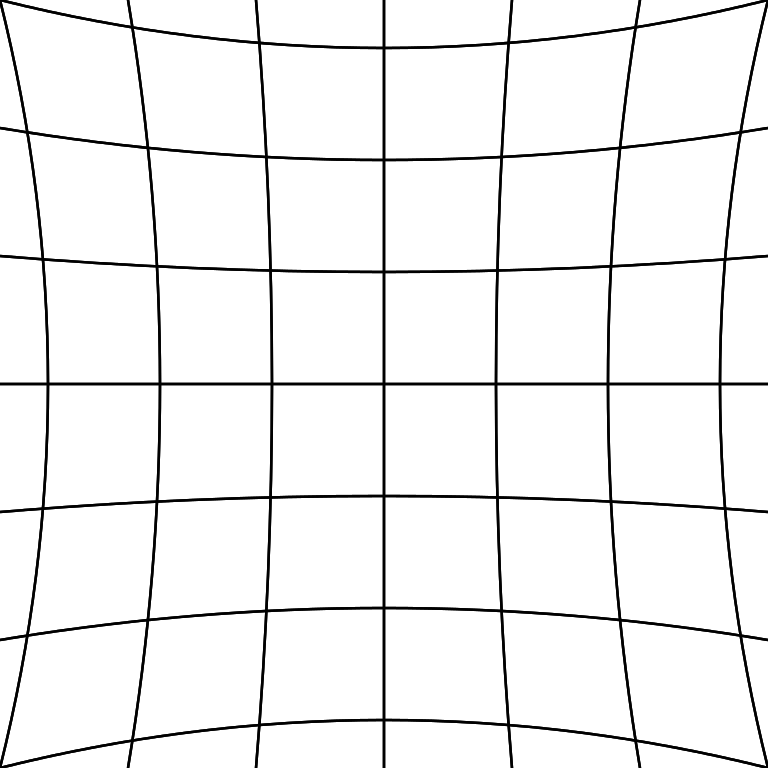
\includegraphics[width=3cm]{pincushion_distortion.png}
			      \caption{Distortion en coussinets (<<pincushion distortion>>)}\par\medskip
			    

			    Pour contrebalancer cette distortion, le programme doit, comme énoncé plus haut, appliquer
			    un effet post-rendu. Il s'agit d'une distortion égale et opposée, appelée distortion en 
			    barillets.\par\bigskip
			    
			     {
			      \centering
				
\includegraphics[width=3cm]{barrel_distortion.png}
			      \caption{Distortion en barillets (<<barrel distortion>>)}
			     }\par\medskip
			    
			    De plus, le programme doit corriger les aberrations chromatiques, qui consistent en un effet
			    d'arc en ciel aux contours des objets. Cet effet est causé par les lentilles.\par\bigskip
			    
			   {
			      \centering
				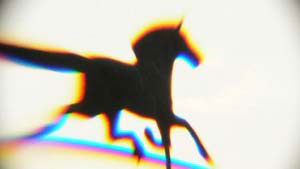
\includegraphics[width=4cm]{chromatic_aberration.jpg}
			      \caption{Aberration chromatique (<<chromatic abberration>>)}
			   }
			    \end{figure}  ~ \\
			    
			    
			\paragraph{Pratique} ~\\
			
			    Pour le développeur, ces éléments théoriques sont gérés de manière interne par le SDK Oculus.
			    
			    Pour une application qui fait un rendu graphique, la programme est typiquement de
			    la forme:\\
			    
			    \begin{algorithm}[H]
			      initialize the graphic resources\;
			      fill the scene with graphic objects\;
			      \While{the application is running}{
				process the user input\;
				update the objects in the scene\;
				render the objects in the scene\;
			      }
			      release the graphic resources\;
			      \caption{Application de rendu graphique}
			    \end{algorithm} ~\\
			    
			   
			    
			    
			    
			    Un programme qui fait un rendu Oculus exclusivement aura pour sa part la forme suivante:\\
			    
			    \begin{algorithm}[H]
			      initialize the graphic resources\;
			      initialize the Oculus SDK\;
			      fill the scene with graphic objects\;
			      \While{the application is running}{
				process the Oculus input\;
				update the objects in the scene\;
				\For{each eye}{
				  translate the camera by the inter-pupillary distance\;
				  apply the Oculus distortion effects\;
				  render the objects in the scene\;
				  }
			      }
			      release the Oculus SDK\;
			      release the graphic resources\;
			      \caption{Application de rendu graphique}
			    \end{algorithm} ~\\
			    Plus précisément, l'opération <<apply the Oculus distortion effects>> se fait de façon graphique
			    au moyen de shaders, qui sont des programmes qui appliquent des transformations à chaque pixel de l'image.
			    
			    
			    Nous avons alors le rendu suivant, pour une scène simple composée d'un cube texturé, d'un plan
			    et d'une skybox rudimentaire, avec le même point de vue:
			    
			    \clearpage
			    
			    \begin{figure}
			      \centering
				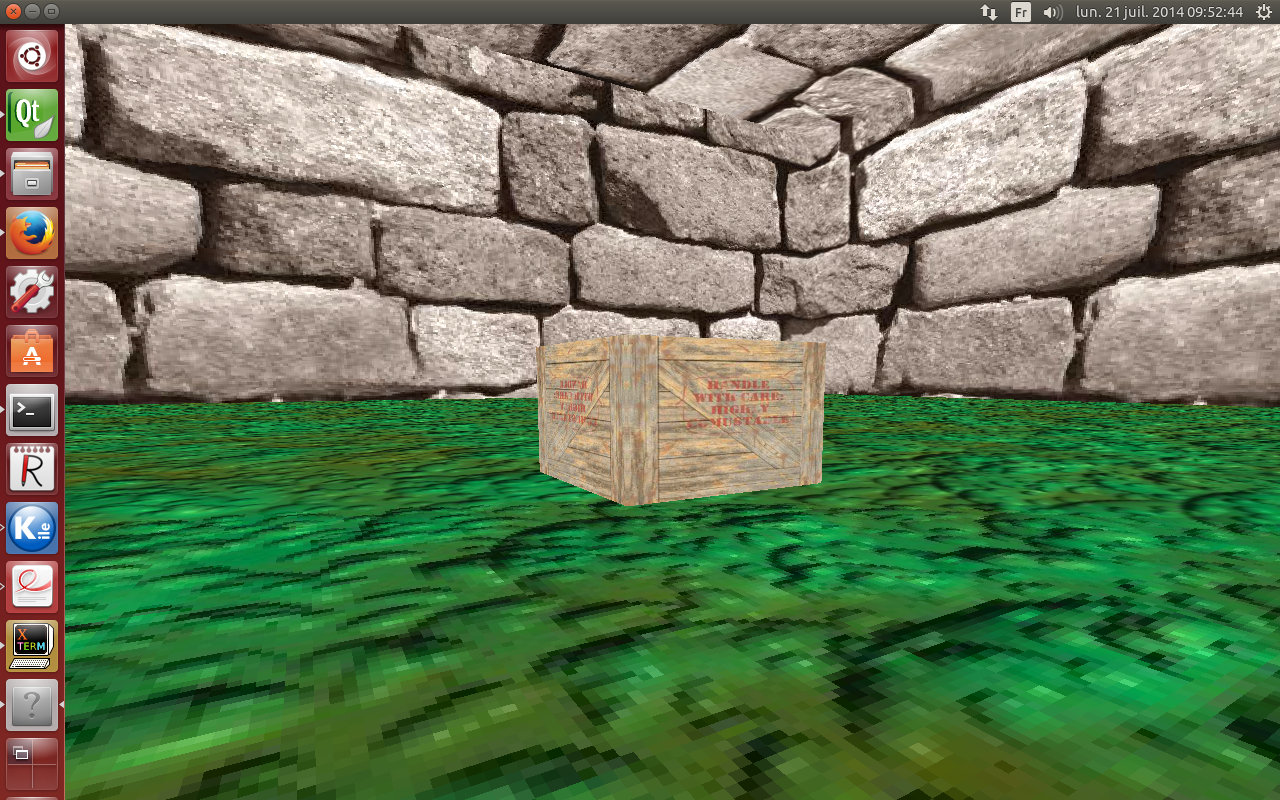
\includegraphics[width=1.0\textwidth]{scene_normal4.png}
			      \caption{Scène OpenGL simple avec le rendu normal}

				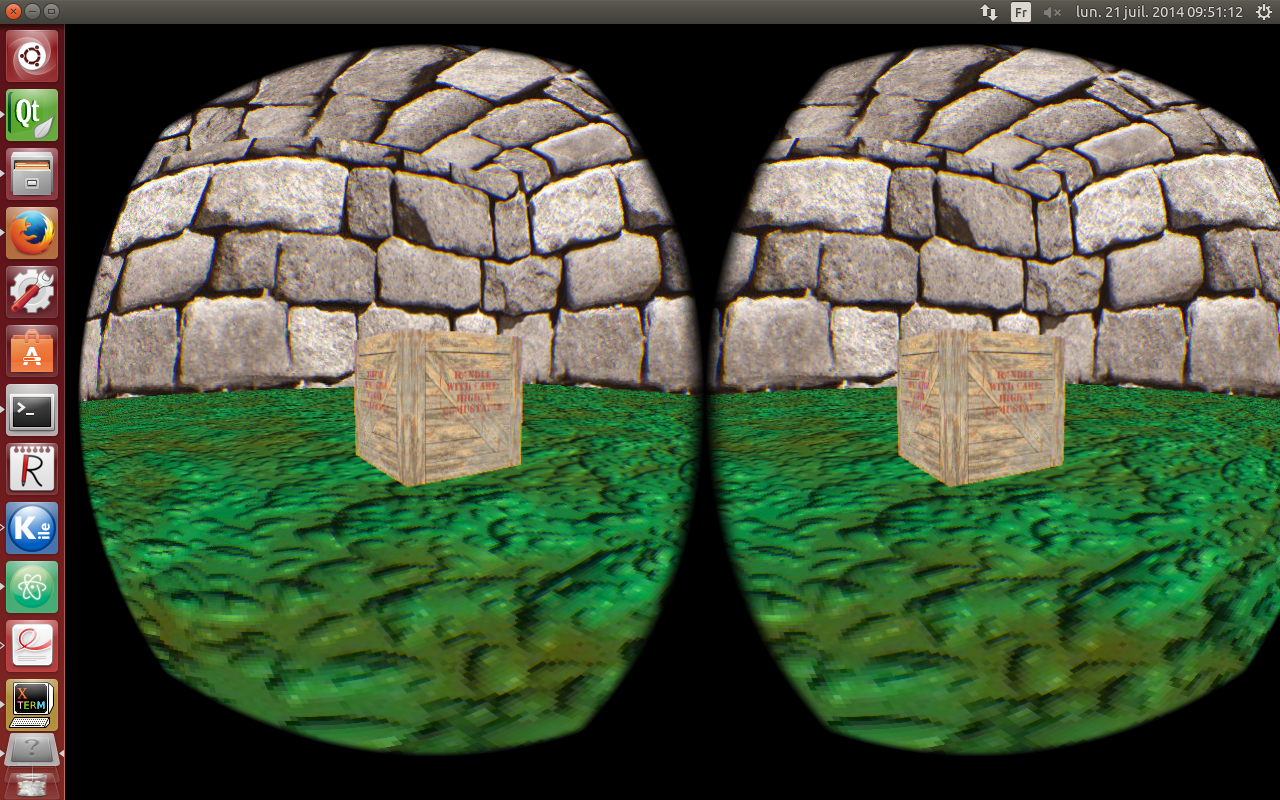
\includegraphics[width=1.0\textwidth]{scene_oculus4.png}
			      \caption{Scène OpenGL simple avec le rendu Oculus}
			    \end{figure}
			    \clearpage
			    
			    
			    
			    
			    Les applications que j'ai développées au sein de mon stage peuvent fournir le rendu normal 
			    et le rendu Oculus, selon l'option spécifiée.

		
	\subsection{Contraintes}
	
	\subsubsection{Skybot 3D}
	    \paragraph{Existant} ~\\
	    
		La contrainte principale pour le projet Skybot 3D a été de travailler avec du code existant non documenté.
		En effet, j'ai eu accès à une version de développement non finalisée et non encore publiée. Cependant j'ai 
		eu de riches échanges avec les développeurs par mail et vidéoconférence.
		
	    \paragraph{Langages} ~\\
	      
		Une contrainte supplémentaire a été le conflit de langages: le programme existant est écrit en C, et le
		SDK Oculus en C++, exigeant en conséquence un compilateur C++. 
		C et C++ sont des langages proches de par leur origine et leur histoire, C++ étant issu de C, 
		ils sont donc en grande partie compatibles. La majorité du code n'a donc pas posé de problème, 
		mais certains motifs ont dû être modifiés, notamment les conversions de types implicites,
		les arithmétiques de pointeurs et les pointeurs de fonctions ont du être réécrits de manière
		idiomatique en C++.
		
	    \paragraph{Versions d'OpenGL} ~\\
	    
		Une contrainte additionnelle, et peut-être la plus importante, a été l'utilisation de différentes 
		fonctionnalités d'OpenGL, appartenant à des versions différentes.
		En effet, la totalité du rendu graphique dans l'application existante se fait avec le <<fixed pipeline>> 
		d'OpenGL, c'est-à dire une suite d'opérations fixes de rendu. Cela consiste a faire un rendu graphique basé sur des
		appels à des fonctions OpenGL qui fournissent des fonctionnalités bien pratiques, comme des transformations
		matricielles, des lumières, \ldots. Cependant ces appels, typiques d'OpenGL 1.x et 2.x, 
		utilisent principalement le CPU et ont donc
		été dépréciés pour des raisons de performances dans OpenGL 3.x et 4.x, au profit d'une programmation
		<<tout shader>>. Les shaders sont des programmes appliquant des effets sur chaque pixel de l'image et qui
		sont éxecutés sur la carte graphique.
		
		Le développeur doit donc maintenant tout faire manuellement mais cela au profit des performances et de l'éventail
		de possibilités, mais au détriment de la simplicité.
		
		Le SDK Oculus utilise les shaders pour appliquer les effets graphiques mentionnés plus tôt (distortion, 
		correction des aberrations, \ldots), et cela a créé quelques conflits au niveau du rendu graphique, 
		avec le rendu existant n'utilisant pas ces shaders.
		
	    \subsubsection{Simulation}
		\paragraph{Portabilité} ~\\
		
		
		  Pour ce projet, il a été convenu dès le départ d'assurer la portabilité du programme, c'est-à-dire
		  le fonctionnement multi-plateforme.
		  
		  Dans cette optique, j'ai choisi un langage fonctionnant sur n'importe quelle plateforme existante 
		  (dès lors qu'il existe un compilateur adéquat), le C++, et
		  des bibliothèques multi-plateformes, notamment pour le rendu graphique,
		  pour permettre l'abstration d'une API spécifique à une plateforme donnée, en fournissant une API générique.
		  Un exemple est l'utilisation de la SDL, une bibliothèque de fenêtrage, ou d'OpenGL, une API de rendu
		  graphique.
		  
		  De plus, un soin particulier a été porté dans le développement à  l'évitement de l'introduction 
		  de code spécifique à une plateforme donnée, par exemple en utilisant de façon maximale la libraire 
		  standard du langage.
		  
		  
		\paragraph{Taille des données} ~\\
		
		  Comme évoqué plus haut, j'ai travaillé sur des données avoisinant le million d'objets. Cela a posé
		  principalement un problème de performances. En effet, c'est en travaillant avec de tels nombres que
		  l'on se rend compte de la disparité CPU (processeur) / GPU (carte graphique).
		  En effet, malgré un processeur avec 16 GB de RAM, le fait de parcourir tous les objets pour les afficher (une fois par frame),
		  prenait plus de 16 millisecondes, nombre critique dans le domaine du rendu graphique, puisqu'il
		  correspond au temps de rendu maximal d'une frame si l'on veut un rendu à 60 FPS (frame per seconds),
		  ce qui fournit une expérience correcte pour l'utilisateur: $1000 ms / 60 = 16.666 ms$.
		  
		  En sus, comme j'ai travaillé avec cubes de données (corps celéstes dont les cooordonnées spatiales se trouvent toutes
		  contenues dans un cube, typiquement de taille 64*64*64 ou 100*100*100), ce qui peut donner une boucle de rendu
		  de complexité $\mathcal{O}(n^3)$, empirant alors le temps de rendu.
		  
		  De plus, il faut garder à l'esprit que l'objectif final est d'avoir un rendu Oculus valide. Or le
		  SDK Oculus fait un double rendu (un pour chaque oeil), en appliquant des transformations matricielles
		  pour chacun des rendus. Il est donc primordial d'avoir des FPS corrects dans le rendu graphique normal.
		  
		  Cependant, je me suis aperçu que la carte graphique ne rencontrait pas de problème de temps de rendu,
		  gardant la plupart du temps un temps de rendu d'une frame inférieur à la milliseconde.
		  
		  Dès lors, plusieurs solutions se sont présentées:
		  
		  \begin{description}
		   \item [Travailler avec un seul objet graphique]~\\ Cela consiste à avoir un seul objet dans le programme qui 
		   contient les coordonnées de tous les objets célestes. On boucle donc sur un seul objet et on envoie toute
		   les positions des objets célestes en une seule fois comme s'il n'y avait q'un objet et la carte
		   graphique fait tout le travail. Cela fonctionne mais est peu flexible (comment faire pour sélectionner
		   un seul objet céleste pour afficher des informations à son sujet?) et on atteint les limites de la
		   carte graphique pour un très grand nombre d'objets.
		   
		   \item [Octree]~\\ Un Octree est un arbre où chaque noeud (appelé <<octant>>) compte jusqu'à 8 fils. Il correspond à partition
		   d'un espace cubique, à la manière d'un quadtree en 2D, et permet de diviser notre scène en régions,
		   contenant elles-mêmes des sous-régions et ainsi de suite. On peut alors décider d'afficher seulement les
		   régions voisines de notre position sans afficher les régions que l'on ne peut pas voir ou qui sont
		   trop lointaines. C'est la solution que j'ai choisie car c'est la plus flexible et celle qui offre le
		   plus de possibilités. A noter cependant que cela impose une taille de cube d'une puissance de deux.
		   
		   \begin{figure}
			      \centering
				\includegraphics[width=0.5\textwidth]{octree.png}
			      \caption{Schématisation d'un octree}
			       
		    \end{figure} 
		    
		
			       
		\begin{figure} 
			\centering
				\includegraphics[width=0.4\textwidth]{octree2.jpg}
			      \caption{Octree en action}
		   
		\end{figure}
		   
		 \end{description}

		  
		 On optimise alors le rendu à la fois sur le CPU (moins d'objets parcourus dans la boucle
			       de rendu à chaque frame) et sur le GPU (moins de données envoyées et 
			       rendues graphiquement à chaque frame).  
		  		
		
		Initialement, mes objets étaient tous stockés dans un tableau que je parcourais à chaque frame pour les afficher.
		Pour 1000 objets, j'avais une moyenne de 5 FPS. 
		J'ai alors mis en place un Octree. J'ai eu alors des FPS variant entre 30 et 60 FPS, avec une moyenne de 55 FPS
		(le rendu est limité à 60 FPS maximum
		pour ne pas surcharger le CPU/GPU), quelque soit le nombre d'objets présents dans la scène, ce qui est acceptable.
		En effet, l'Octree permet d'afficher un nombre moyen constant d'objets quelque soit notre position.
		Avec un cube de taille 128*128*128 et 32768 objets, le temps de génération de l'Octree est d'environ 120s.
		J'affiche l'octant (et donc tous les objets célestes se trouvant dans cet octant) où la caméra se trouve
		et les 6 octants immédiatement voisins, avec une taille d'octant de 8.
		Pour résumer, on sacrifie le temps de démarrage du programme au profit des performances à l'exécution.


	\subsection{Outils utilisés}

		\subsubsection{Langages utilisés}
		    Les deux projets sur lesquels j'ai travaillé ont été développés en C++, même si la quasi-totalité 
		    du projet Skybot 3D est écrite en C, adapté pour pouvoir compiler en C++.
		    Sur le deuxième projet, j'ai de plus mis en oeuvre des fonctionnalités nouvelles de C++, standardisées
		    par la norme C++11 datant de 2011. On peut citer:
		    \begin{itemize}
		     \item Listes d'initialisation 
		     \item Pointeur null <<nullptr>>
		     \item Boucle for sur une plage de valeurs
		     \item Référence sur une rvalue
		     \item Outils de mesure du temps
		     \item Mot-clé <<auto>>
		    \end{itemize}
	
		\subsubsection{Bibliothèques utilisés}

		  \begin{description}
		   \item [OpenGL] ~\\
		      OpenGL est une API multi-plateforme pour effectuer des rendus graphiques 2D et 3D.
		      L'implémentation est laissée à la charge des constructeurs de cartes graphiques et est fournie
		      par les drivers. Pour ma part j'ai travaillé avec la carte graphique AMD Radeon HD 8570 disposant d'1Gb de RAM dédiée  
		      et le driver ATI Fire GL datant de mai 2014, implémentant OpenGL 4.4 (dernière version d'OpenGL).
		      
		      Je l'ai utilisée pour les deux projets.
		      
		   \item [SDL]~\\
		      <<Simple DirectMedia Layer>> est une bibliothèque multi-plateforme donnant accès au système de fenêtrage,
		      au clavier, à la souris et à un éventuel joystick. Je l'ai utilisée pour le projet de simulation.
		      
		   \item [GLUT]~\\
		      <<OpenGL Utility Toolkit>> est l'équivalent de la SDL en plus restreint. Je m'en suis servi pour le 
		      projet Skybot 3D via son implémentation open source <<freeglut>>.
		      
		   \item [glm]~\\
		      <<OpenGL Mathematics>> est une bibliothèque de fonctions mathématiques pour OpenGL.
		      Je l'ai utilisée pour le projet de simulation.
		      
		   \item [Oculus SDK]~\\
		      Le SDK Oculus est l'interface de programmation permettant d'accéder à l'Oculus Rift et est fourni
		      par Oculus VR (fabriquant de l'Oculus Rift). 
		      Je me suis servi des versions 0.2.5 et 0.3.2.
		      
		  \end{description}

		
		
		\subsubsection{Programmes utilisés}
		  \begin{description}
		   \item [QtCreator]~\\
		      IDE C++ open source avec débuggeur et outils d'analyses intégrés.
		   
		   \item [Clang]~\\
		      Compilateur/interface de compilation C/C++ open source développé par Google.
		   
		   \item [GCC]~\\
		      <<GNU Compiler Collection>>, compilateur C/C++.
		    
		   \item [Valgrind]~\\
		      Outil d'analyse dynamique (à l'exécution) de programme, pour notamment traquer les fuites de mémoire.
		   
		   \item [Clang Static Analyzer]~\\
		      Outil d'analyse statique (à la compilation) de code et qui fait partie du projet Clang.
		   
		  \end{description}

		
		
	\subsection{Déroulement du stage}
	
		%Déroulement
	
	\subsection{Bonnes pratiques de développement}
			%Bonnes pratiques
	
	\subsection{Architecture}
	
  %Architecture de l'application

			
\section{Remerciements}

	Plusieurs personnes m’ont apporté une aide significative sur ce projet et je tiens à les remercier chaleureusement ici: 

	\begin{itemize}
	 \item André SCHAAF, mon maître de stage
	 \item L'équipe Skybot 3D: Jérôme Berthier et Jonathan Normand
	 \item Brad Davis, auteur du livre <<Oculus Rift in Action>>, pour l'aide qu'il m'a apporté sur les forums d'Oculus Rift
	 \item Nicolas Deparis et Romain Houpin, stagiaires à l'Observatoire sur des sujets de rendu graphique 3D
	\end{itemize}


  
  
\section{Conclusion}


		%Conclusion

% \appendix
\section{Annexes}
	
		\subsection{Captures d'écran}
		\newpage
		%Captures d'écran
	
	
	\subsection{Bibliographie}
	
		%Bibliographie

		
	\subsection{Glossaire}
		%Glossaire
		
\end{document}

